\documentclass[10pt]{article}

\usepackage[T1]{fontenc}
\usepackage{geometry}
\usepackage{amsmath, amssymb, amsthm}
\usepackage{xcolor}
\usepackage{graphicx}
\usepackage{float}
\usepackage{caption}
\usepackage{subcaption}
\usepackage{listings}
\usepackage{hyperref}

\geometry{a4paper, margin=1in}

\newcommand{\C}{\mathbb{C}}
\newcommand{\R}{\mathbb{R}}
\newcommand{\Q}{\mathbb{Q}}
\newcommand{\Z}{\mathbb{Z}}
\newcommand{\N}{\mathbb{N}}

\definecolor{codegreen}{rgb}{0,0.6,0}
\definecolor{codegray}{rgb}{0.5,0.5,0.5}
\definecolor{codepurple}{rgb}{0.58,0,0.82}
\definecolor{backcolour}{rgb}{1,1,1}

\lstdefinestyle{mystyle}{
    backgroundcolor=\color{backcolour},
    commentstyle=\color{codegreen},
    keywordstyle=\color{blue},
    stringstyle=\color{codepurple},
    basicstyle=\ttfamily\footnotesize,
    breakatwhitespace=false,
    breaklines=true,
    keepspaces=true,
    numbers=left,
    numbersep=5pt,
    showspaces=false,
    numberstyle=\ttfamily\footnotesize\color{codegray},
    showstringspaces=false,
    showtabs=false,
    tabsize=4
}

\lstset{style=mystyle}

\title{
    \Large\textsc{MA3206: Statistics I} \\
    \Huge \textbf{Estimating $\pi$ by rejection sampling} \\
    \vspace{5pt}
    \Large{Spring 2022}
}
\author{
    \large Satvik Saha
    \\\textsc{\small 19MS154}
}
\date{\normalsize
    \textit{Indian Institute of Science Education and Research, Kolkata, \\
    Mohanpur, West Bengal, 741246, India.} \\
}

\begin{document}
    \maketitle

    \tableofcontents

    \section{Problem statement}
    
    Consider the unit disc, \[
        D = \{(x, y) \in \R^2 : x^2 + y^2 \leq 1\},
    \] and the ellipse \[
        D' = \{(x, y) \in \R^2 : 2(x - 1)^2 + 5(y - 2)^2 \leq 8 \}.
    \] The task is to sample some $n$ points from $D$ and $D'$, and thereby estimate
    the value of $\pi$. For reference, \[
        \pi = 3.141592653589793 \dots
    \] 


    \section{Rejection sampling}

    Consider a region $A \subset \R^2$, from which we want to sample points
    uniformly. In other words, we want to simulate the probability density function
    \[
        u_A\colon \R^2 \to \R, \qquad u_A(x, y) = \frac{1}{\mu(A)}\chi_A(x, y) = \begin{cases}
            1 / \mu(A), &\text{ if } (x, y) \in A, \\
            0, &\text{ otherwise}.
        \end{cases}
    \] Here, for $E \subseteq \R^2$, we denote \[
        \mu(E) = \int_E\:dx\:dy,
    \] the `area' or measure of $E$. Now suppose that $A$ is enclosed within a
    rectangle $R = [a, b] \times [c, d]$. We can simulate a uniform distribution on
    $R$ easily enough, by sampling individual coordinates $x \in [a, b]$, $y \in [c,
    d]$ uniformly. This means that we can simulate the probability density function
    \[
        u_R\colon \R^2 \to \R, \qquad u_R(x, y) = \frac{1}{\mu(R)}\chi_R(x, y) = \begin{cases}
            1 / \mu(R), &\text{ if } (x, y) \in R, \\
            0, &\text{ otherwise}.
        \end{cases}
    \] Note that we have normalized \[
        \int_{\R^2} u_A(x, y)\:dx\:dy = \int_{\R^2} u_R(x, y)\:dx\:dy = 1.
    \] Also, $\mu(R) = (b - a)(d - c)$.

    In order to simulate the distribution $u_A$, we propose rejection sampling
    from $u_R$. In other words, draw a point $(x, y) \in R$ using the distribution
    $u_R$. If $(x, y) \in A$, accept this as a sample point; if not, reject it.
    Repeat this process of drawing points from $R$ and checking until we have all $n$
    sample points.

    Consider a point $(X, Y) \in R$ drawn using the distribution $u_R$. We
    compute the probability that it is accepted as follows. \begin{align*}
        P[(X, Y) \text{ accepted}] &= \int_R P[(X, Y)\text{ accepted} \mid X = x, Y =
        y]\, u_R(x, y)\:dx\:dy \\
        &= \int_R \chi_A(x, y)\,u_R(x, y)\:dx\:dy \\
        &= \int_A \frac{1}{\mu(R)}\:dx\:dy \\
        &= \frac{\mu(A)}{\mu(R)}.
    \end{align*}
    The second line follows from the fact that $(X, Y)$ is accepted if and only if
    $(X, Y) \in A$. This result aligns well with our intuition that the probability
    of acceptance ought to be the ratio of areas of $A$ and $R$. If $N$ points are
    drawn from $R$ out of which $n$ were accepted, we approximate \[
        P[(X, Y) \text{ accepted}] = \frac{\mu(A)}{\mu(R)} \approx \frac{n}{N}.
    \]

    Now, we show that points sampled in this way are indeed distributed uniformly
    over $A$, as in $u_A$. Let $E\subseteq A$ be an arbitrary (measurable) region.
    Consider an accepted point $(X, Y) \in A$ in our sample. Using Bayes' Theorem,
    we have \[
        P[(X, Y) \in E \mid (X, Y) \text{ accepted}] = P[(X, Y) \text{ accepted} \mid
        (X, Y) \in E]\cdot \frac{P[(X, Y) \in E]}{P[(X, Y) \text{ accepted}]}.
    \] Note that $(X, Y)$ is always accepted if $(X, Y) \in E$ \subseteq A. Also,
    $(X, Y)$ was chosen uniformly from $R$ using $u_R$, so we can compute much like
    before
    \begin{align*}
        P[(X, Y) \in E] &= \int_R P[(X, Y) \in E\mid X = x, Y = y]\, u_R(x,
        y)\:dx\:dy \\
        &= \int_R \chi_E(x, y)\,u_R(x, y)\:dx\:dy \\
        &= \int_E \frac{1}{\mu(R)}\:dx\:dy \\
        &= \frac{\mu(E)}{\mu(R)}.
    \end{align*}
    Putting things together, \[
        P[(X, Y) \in E \mid (X, Y) \text{ accepted}] = \frac{\mu(E)}{\mu(R)}\cdot
        \frac{\mu(R)}{\mu(A)} = \frac{\mu(E)}{\mu(A)}.
    \] However, this is precisely the defining property of the uniform distribution
    on $A$ described by $u_A$; the probability of a sample point $(X, Y)$ lying
    within an arbitrary region $E \subseteq A$ being proportional to the area of $E$.
    Thus, our sample obtained in this way does indeed follow distribution $u_A$.


    \subsection{The unit disc}

    The unit disc $D$ is enclosed within the square $S = [-1, 1] \times [-1, 1]$.
    Thus, we can calculate the areas $\mu(D) = \pi$, $\mu(S) = 4$. By setting $A =
    D$, $R = S$, we can use the outlined method to draw sample points uniformly from
    $D$. If $n$ samples points are obtained over $N$ draws, we approximate \[
        \frac{\pi}{4} \approx \frac{n}{N}.
    \] 


    \subsection{The ellipse}
    
    By rewriting the defining equation for $D'$ as \[
        \frac{(x - 1)^2}{4} + \frac{(y - 2)^2}{8 / 5} \leq 1,
    \] it is clear that this is an elliptical region centred at $(1, 2)$, with major
    and minor axes parallel to the $x$ and $y$ axes respectively. Furthermore, the
    semi-major and semi-minor axes have lengths $2$ and $\sqrt{8 / 5}$ respectively.

    The ellipse $D'$ is thus enclosed within the square $S' = [-1, 3] \times [0, 4]$.
    We can calculate the areas $\mu(D') = \pi\cdot 2 \cdot \sqrt{8 / 5}$, $\mu(S') =
    16$. By setting $A = D'$, $R = S'$, we can use the outlined method to draw sample
    points uniformly from $D'$. If $n$ samples points are obtained over $N$ draws, we
    approximate \[
        \frac{\pi\cdot 2 \cdot \sqrt{8 / 5}}{16} = \frac{\pi}{\sqrt{40}} \approx
        \frac{n}{N}.
    \] 


    \section{Algorithm}
    
    In summary, here is the algorithm used to sample $n$ points from a region $A
    \subset \R^2$ with uniform distribution $u_A$, where $A$ is enclosed within the
    rectangle $R = [a, b] \times [c, d]$.
    \begin{enumerate}
        \item Select $x_i \in [a, b]$ and $y_i \in [c, d]$ uniformly. In other words,
        select $(x_i, y_i)$ uniformly from the rectangle $R$.
        \item Check whether $(x_i, y_i) \in A$. If so, add the point $(x_i, y_i)$ to
        a pile of accepted points, otherwise add it to a pile of rejected points.
        \item Repeat steps 1, 2 until the accepted pile has $n$ points.
        \item Let the total number of points in the accepted and rejected piles be
        $N$. Then, we have $\mu(A) / \mu(R) \approx n / N$.
        \begin{enumerate}
            \item For the unit disc, we use the approximation $\pi \approx 4n/N$.  
            \item For the ellipse, we use the approximation $\pi \approx
            \sqrt{40}n/N$.
        \end{enumerate}
    \end{enumerate}



    \section{Program execution}
    
    \subsection{The unit disc}
    
    The above algorithm for the unit disc has been implemented in the python script
    \texttt{sample\_disc.py}, listed in Sec.~\ref{sec:code_listing}. The script also
    plots the data points for better visualisation.
    
    Below is an execution of the script, with $n = 10$ samples drawn from the unit
    disc. Each line (apart from the summary at the end) shows the $x$ and $y$
    coordinate of the data point, along with whether the point was accepted or
    rejected.

    \begin{lstlisting}[numbers=none, basicstyle=\ttfamily]
        $ ./sample_disc.py 10
          0.73233093  -0.29713792   accepted
          0.34659601   0.05158366   accepted
          0.52026872  -0.75515856   accepted
         -0.22484447  -0.80110737   accepted
          0.32262891  -0.11055622   accepted
          0.52150728  -0.90408779   rejected
         -0.85531360   0.18878968   accepted
         -0.05718717  -0.43605130   accepted
          0.83832780  -0.81159708   rejected
         -0.04045486  -0.97506796   accepted
         -0.25494000   0.36426489   accepted
          0.33717710  -0.13154315   accepted
        10 samples accepted out of 12 draws.
        Estimated value of pi is 3.33333333
        Error is 0.19174068 (6.103295%)
    \end{lstlisting}
    
    \begin{figure}[H]
    \centering
    \begin{subfigure}{0.45\textwidth}
        \centering
        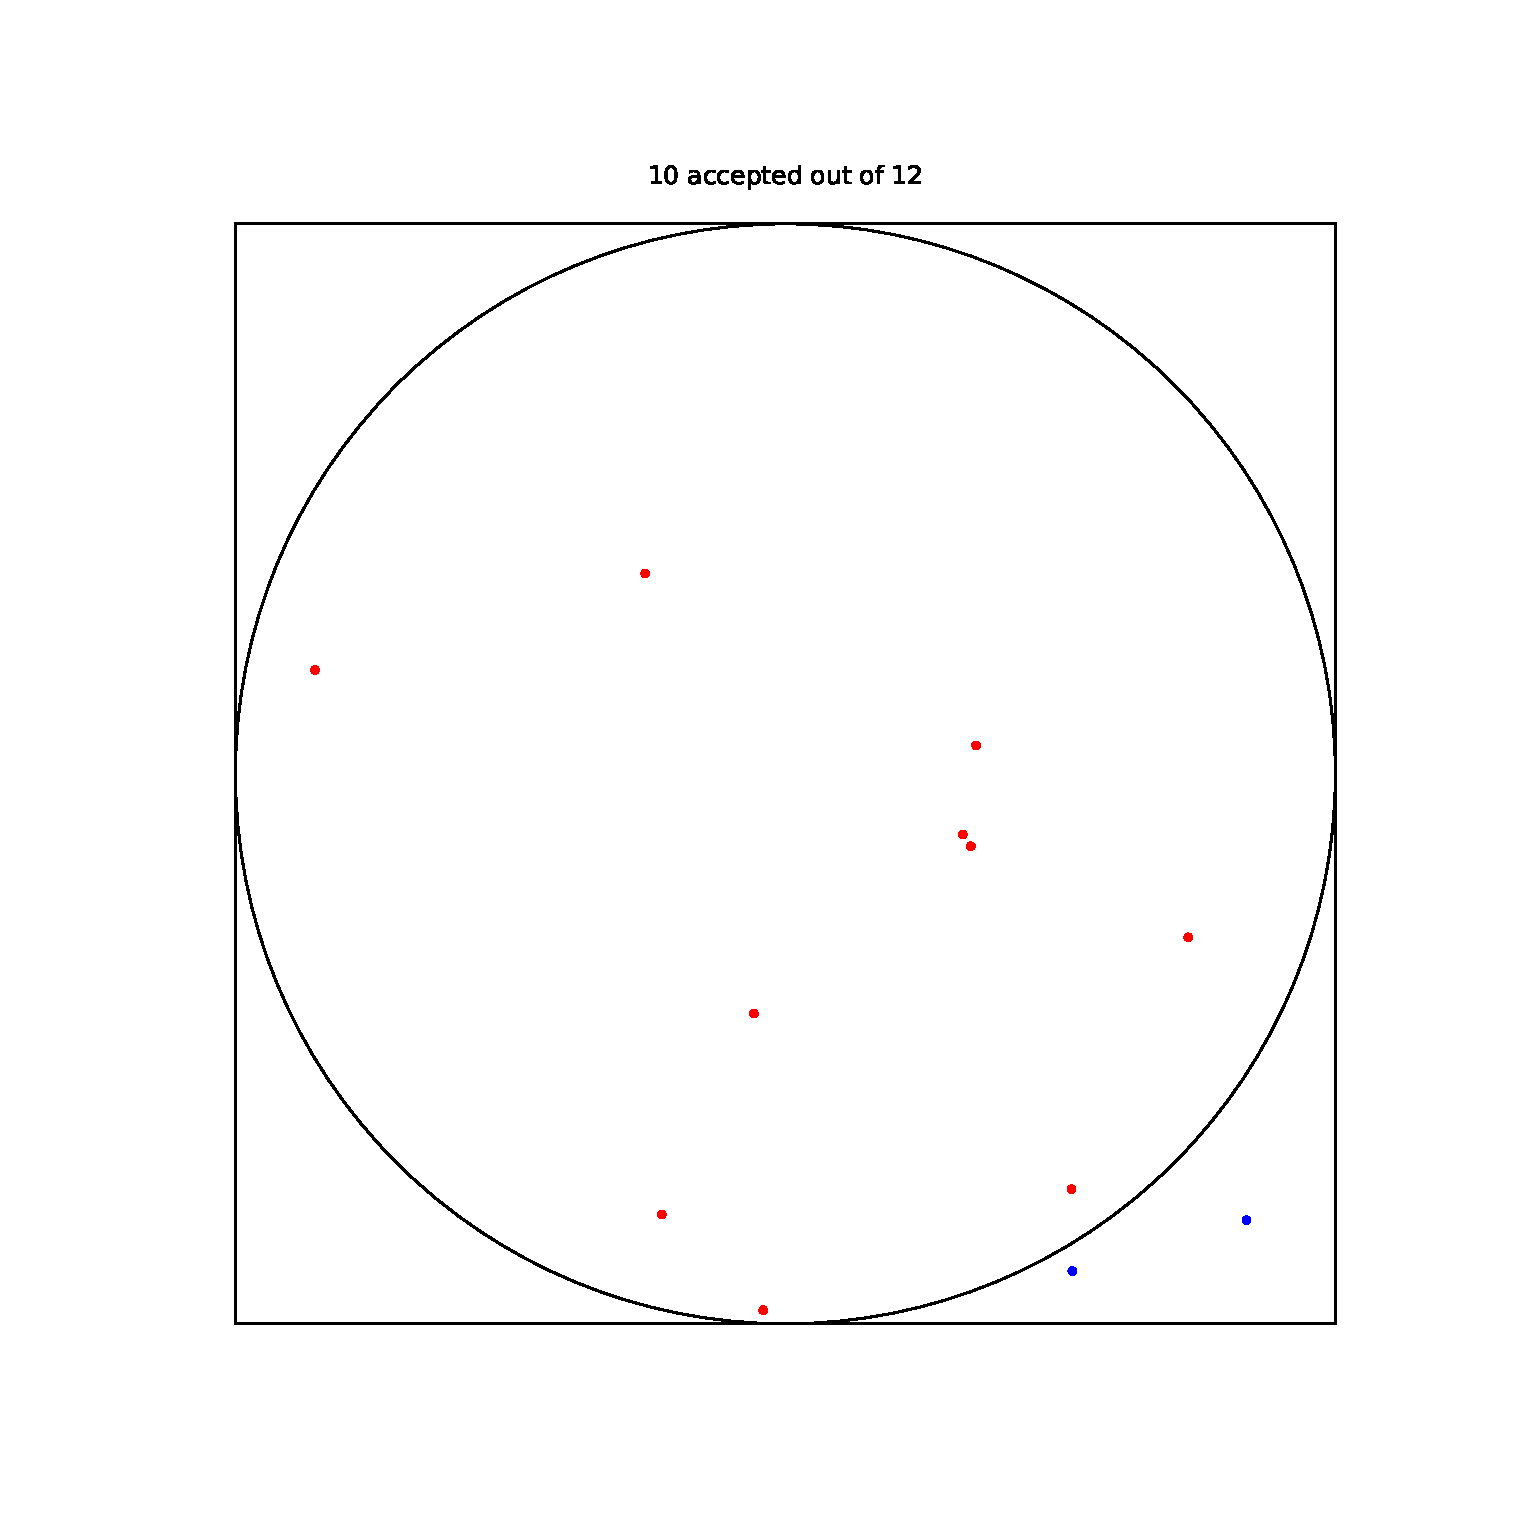
\includegraphics[width=\textwidth, trim=3cm 3cm 3cm 2cm,
        clip]{./points_disc_10.eps}
    \end{subfigure}
    \begin{subfigure}{0.45\textwidth}
        \centering
        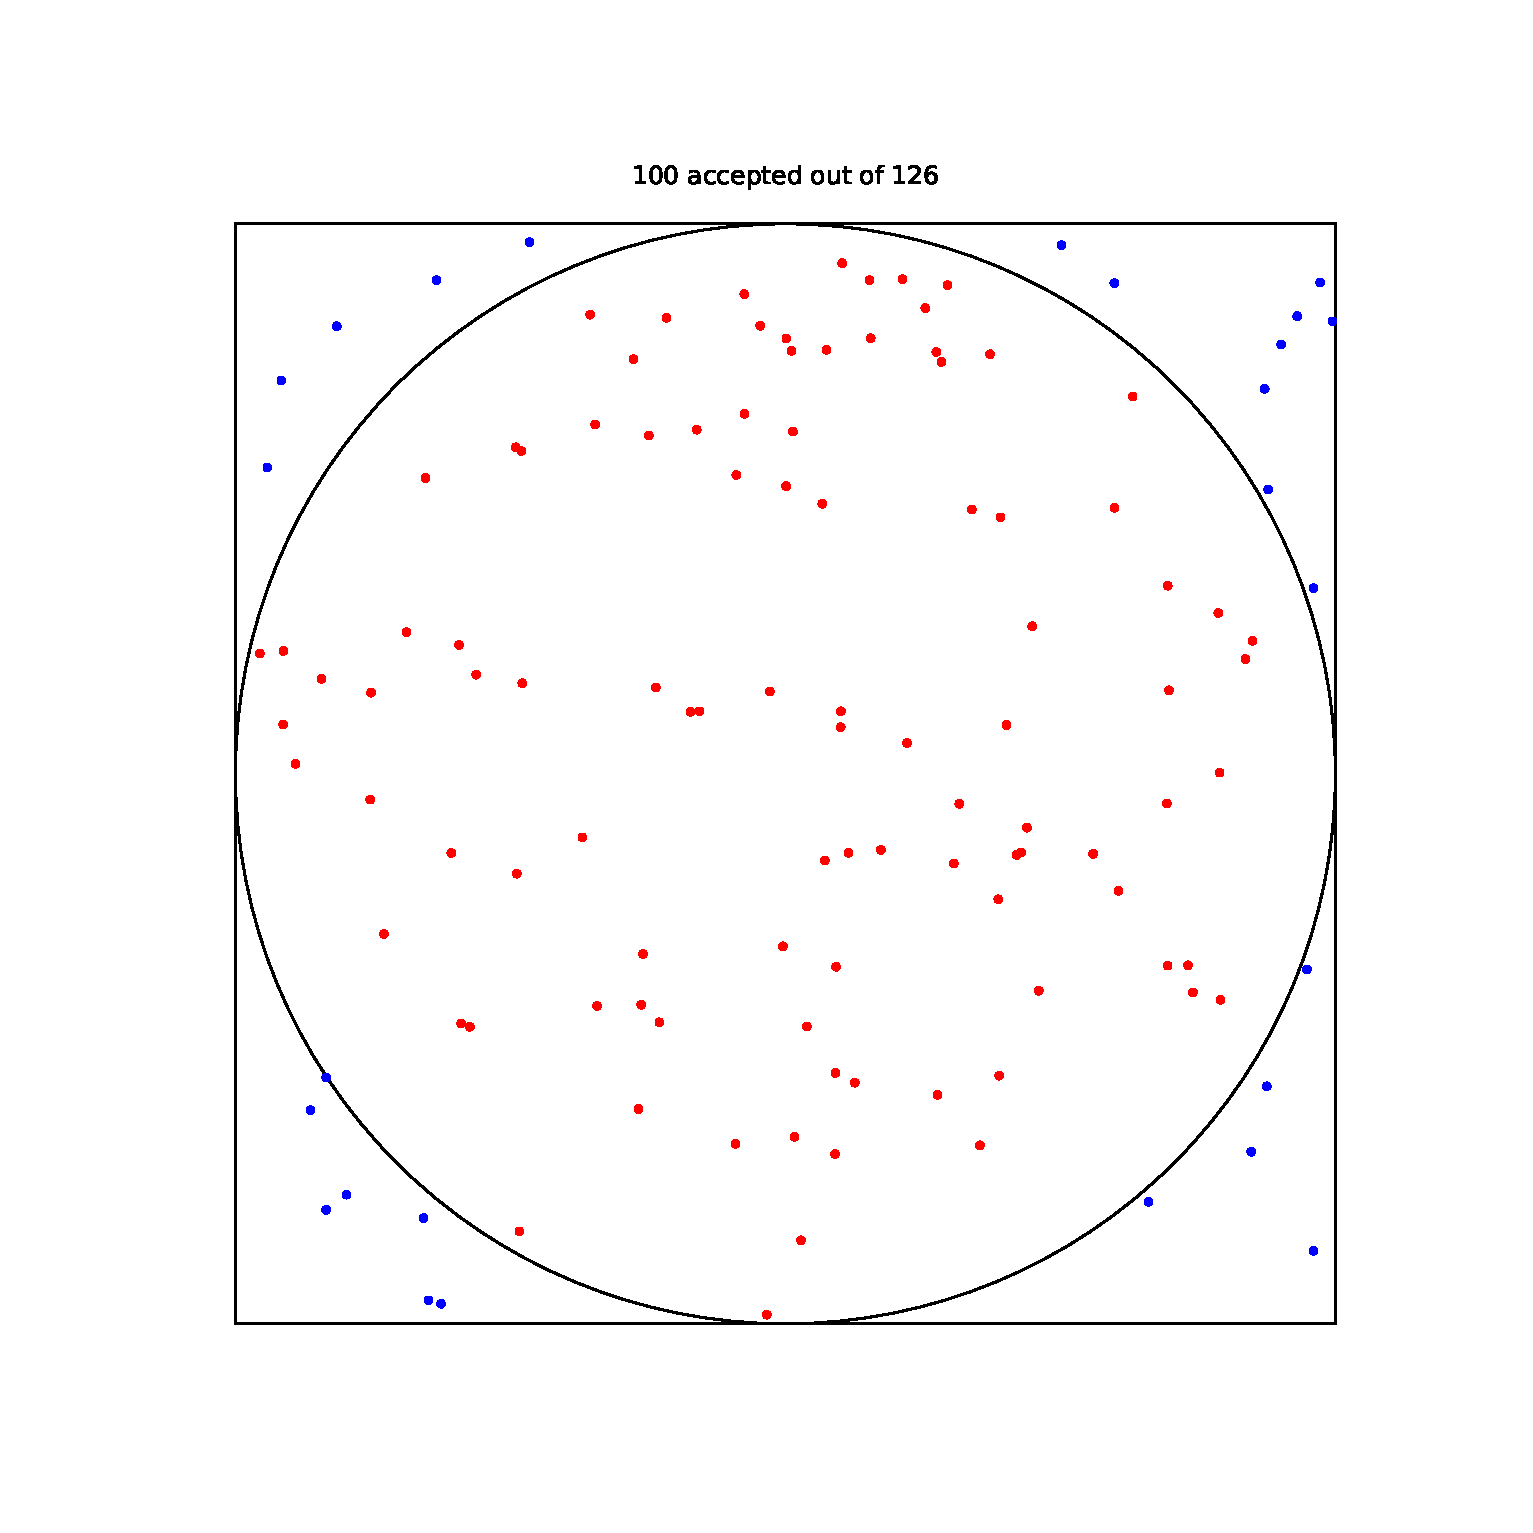
\includegraphics[width=\textwidth, trim=3cm 3cm 3cm 2cm,
        clip]{./points_disc_100.eps}
    \end{subfigure}
    \begin{subfigure}{0.45\textwidth}
        \centering
        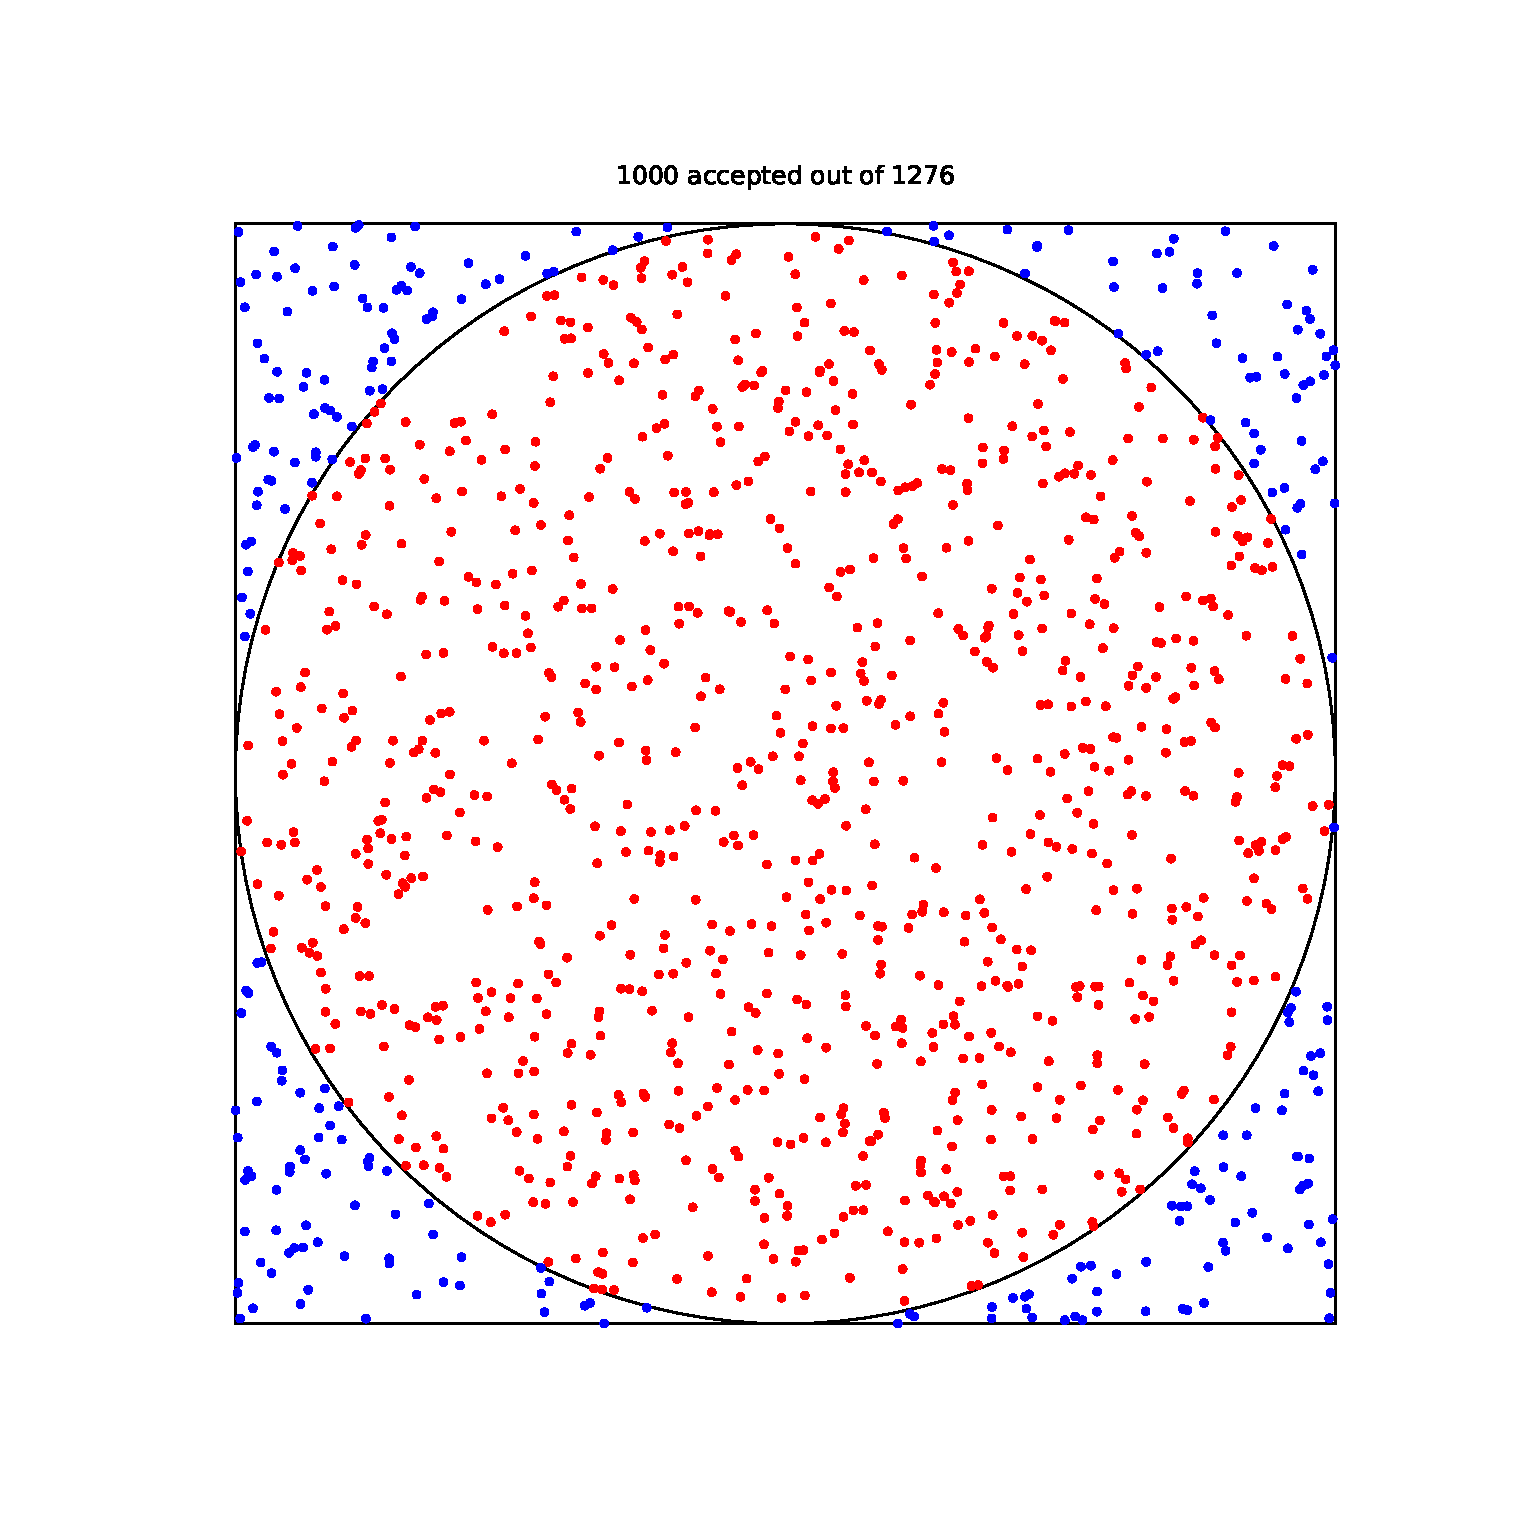
\includegraphics[width=\textwidth, trim=3cm 3cm 3cm 2cm,
        clip]{./points_disc_1000.eps}
    \end{subfigure}
    \begin{subfigure}{0.45\textwidth}
        \centering
        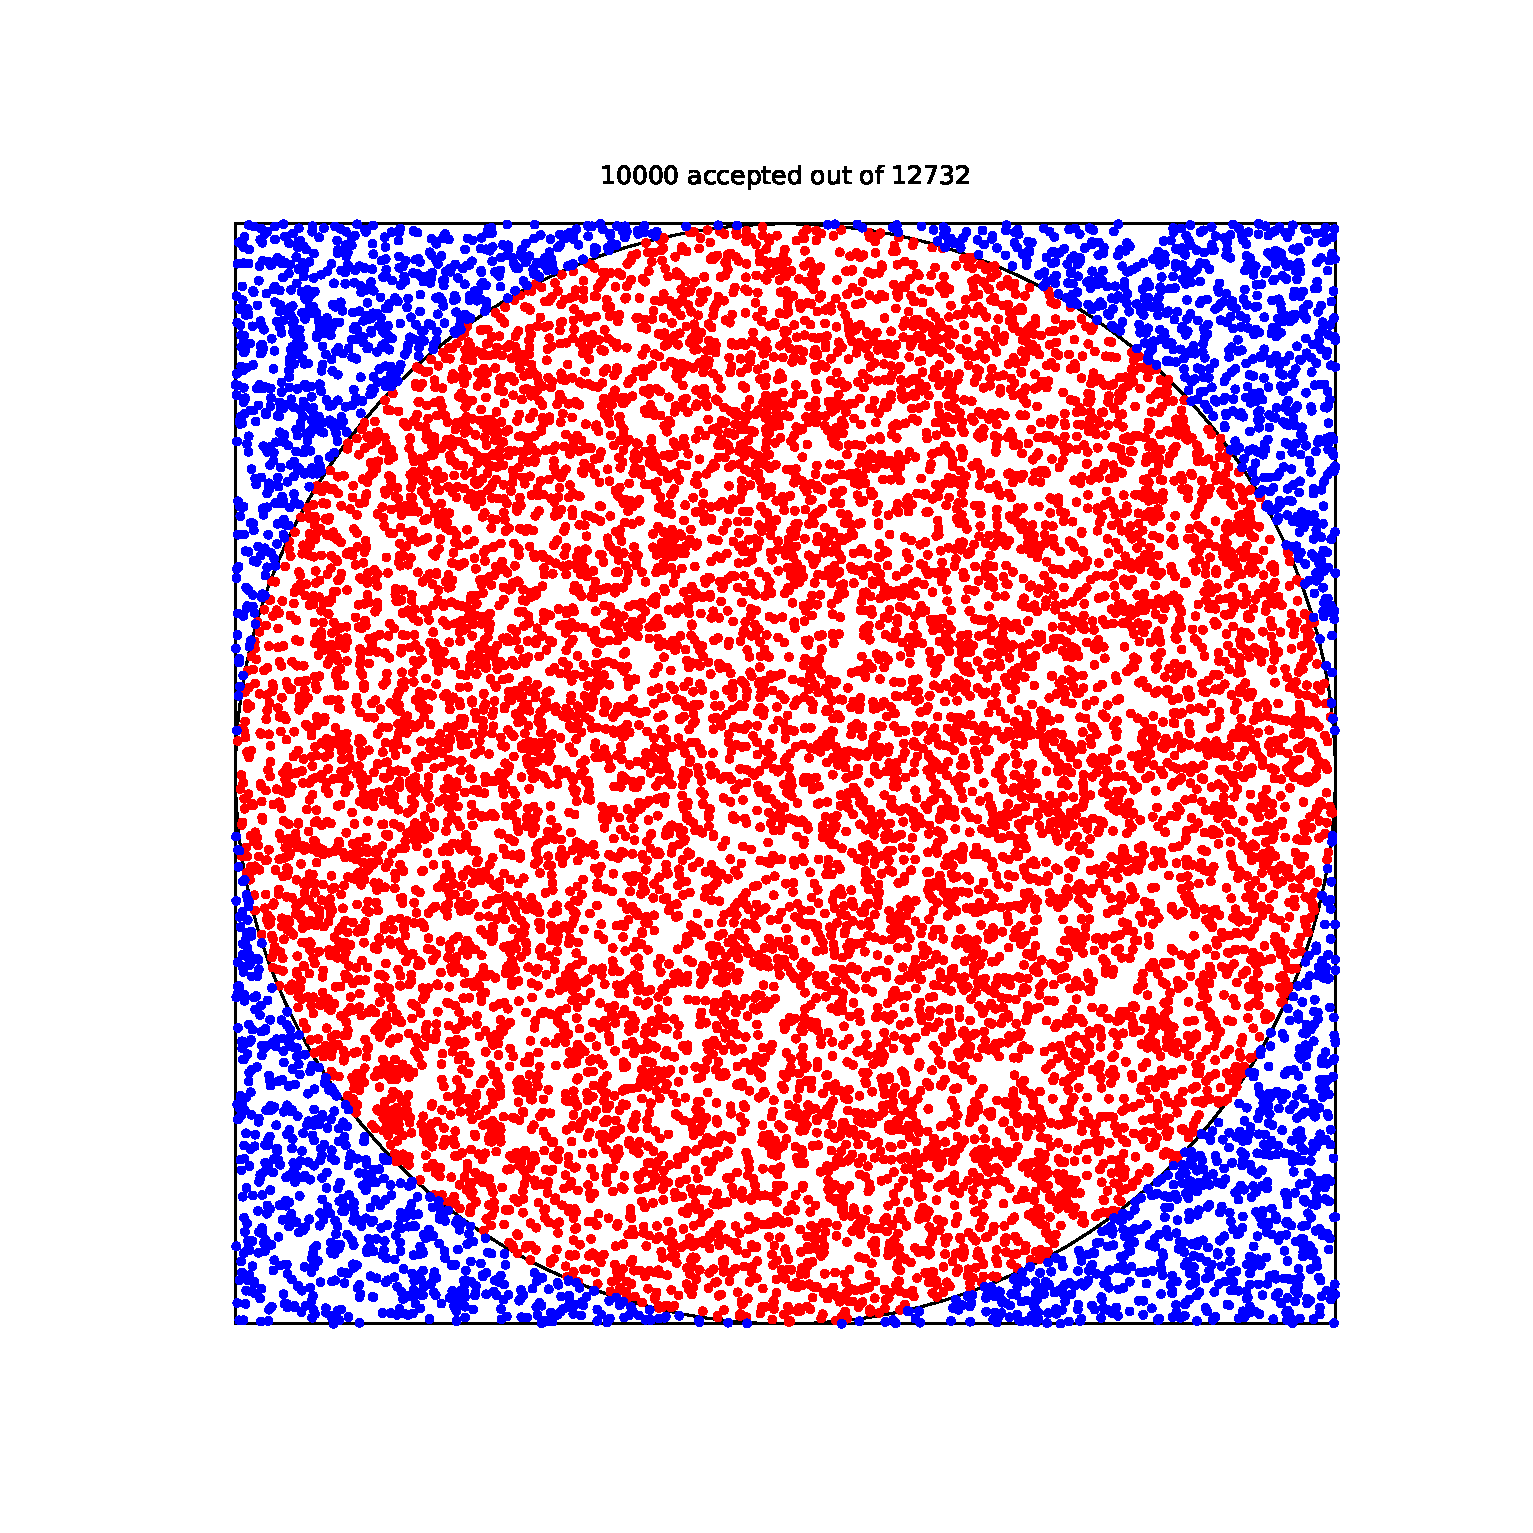
\includegraphics[width=\textwidth, trim=3cm 3cm 3cm 2cm,
        clip]{./points_disc_10000.eps}
    \end{subfigure}
    \caption{Samples drawn from the unit disc in red, rejected points in blue, $n =
    10, 100, 1000, 10000$.}
    \end{figure}

    Following are executions of the script with $n = 100, 1000, 10^4, 10^5, 10^6$
    samples drawn. The data points have been redirected to separate files for
    brevity.

    \begin{lstlisting}[numbers=none, basicstyle=\ttfamily]
        $ ./sample_disc.py 100 2> samples_disc_100.dat
        100 samples accepted out of 126 draws.
        Estimated value of pi is 3.17460317
        Error is 0.03301035 (1.050752%)
        
        $ ./sample_disc.py 1000 2> samples_disc_1000.dat
        1000 samples accepted out of 1276 draws.
        Estimated value of pi is 3.13479624
        Error is -0.00679641 (-0.216337%)

        $ ./sample_disc.py 10000 2> samples_disc_10000.dat
        10000 samples accepted out of 12732 draws.
        Estimated value of pi is 3.14169023
        Error is 0.00009758 (0.003106%)
        
        $ ./sample_disc.py 100000 2> samples_disc_100000.dat
        100000 samples accepted out of 127433 draws.
        Estimated value of pi is 3.13890437
        Error is -0.00268828 (-0.085571%)

        $ ./sample_disc.py 1000000 2> samples_disc_1000000.dat
        1000000 samples accepted out of 1272742 draws.
        Estimated value of pi is 3.14282078
        Error is 0.00122813 (0.039092%)
    \end{lstlisting}
    

    The \texttt{sample\_disc\_mean.py} script performs this sampling process for
    multiple runs, averaging the estimates of $\pi$ from each run, and displaying the
    $\pi$ estimates as a histogram.

    \begin{lstlisting}[numbers=none, basicstyle=\ttfamily]
        $ ./sample_disc_mean.py 1000 1000 2> /dev/null
        Mean of pi estimates from 1000 runs, each with 1000 samples, is 3.142724742209441
        Error is 0.00113209 (0.036035%)
    \end{lstlisting}

    \begin{figure}[H]
    \begin{center}
        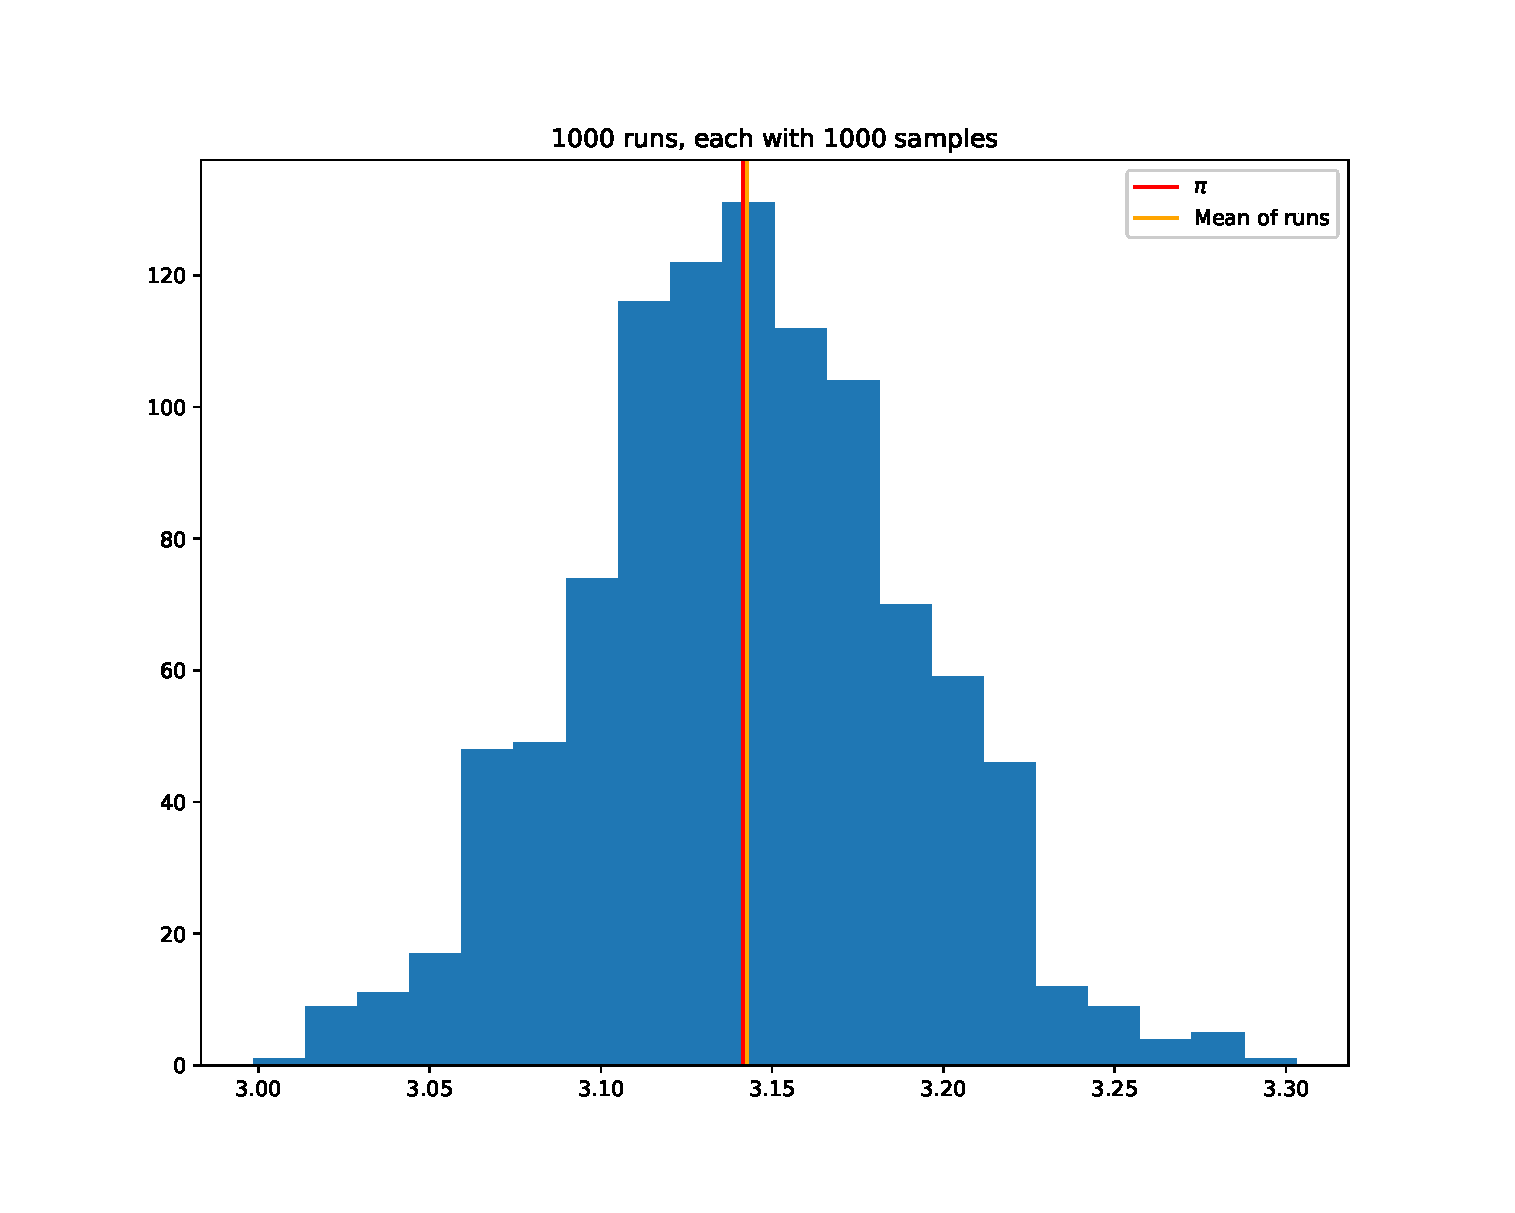
\includegraphics[width=0.8\textwidth]{./runs_hist.eps}
    \end{center}
    \vspace{-4em}
    \caption{Histogram of estimates of $\pi$ obtained from $1000$ runs, each of which
    samples $n = 1000$ points.}
    \end{figure}


    In order to obtain much faster execution speeds, the algorithm for the unit disc
    has also been implemented in the C++ program \texttt{sample\_disc.cpp}, listed in
    Sec.~\ref{sec:code_listing}. Below are a few executions for $n = 10^5, 10^6,
    10^7, 10^8$.
    
    \begin{lstlisting}[numbers=none, basicstyle=\ttfamily]
        $ g++ -o sample_disc sample_disc.cpp
        $ ./sample_disc 100000
        100000 accepted, 127441 total, pi estimated as 3.138707
        Error is -0.002885 (-0.091843%)
        
        $ ./sample_disc 1000000
        1000000 accepted, 1273707 total, pi estimated as 3.140440
        Error is -0.001153 (-0.036700%)

        $ ./sample_disc 10000000
        10000000 accepted, 12733700 total, pi estimated as 3.141271
        Error is -0.000322 (-0.010245%)
        
        $ ./sample_disc 100000000
        100000000 accepted, 127320126 total, pi estimated as 3.141687
        Error is 0.000094 (0.003007%)
    \end{lstlisting}


    \subsection{The ellipse}
    
    The algorithm for the ellipse has been implemented in the python script
    \texttt{sample\_ellipse.py}, listed in Sec.~\ref{sec:code_listing}. The script
    also plots the data points for better visualisation. Below is an execution of the
    script, with $n = 10$ samples drawn from the unit disc.
    
    \begin{lstlisting}[numbers=none, basicstyle=\ttfamily]
        $ ./sample_ellipse.py 10
          2.17950199   3.73800320   rejected
          1.08590943   1.97214632   accepted
         -0.72460138   0.29850537   rejected
          0.14060985   3.13547978   accepted
          2.43026007   0.00517840   rejected
          1.69725367   0.37317408   rejected
          2.98606978   2.04202534   accepted
         -0.75396791   1.43706716   accepted
          2.02528250   1.24398366   accepted
         -0.57610408   0.60839471   rejected
          0.65326239   3.43285296   rejected
          2.02370550   2.07640832   accepted
          2.71615959   0.07882299   rejected
          2.75012591   3.90455867   rejected
          2.35430809   0.99566044   rejected
          1.04111028   0.61737784   rejected
         -0.25423444   2.30809614   accepted
         -0.52347198   3.03817098   rejected
          1.97866215   0.44457484   rejected
          0.27278245   1.30040501   accepted
          1.38116679   1.38268388   accepted
          2.71280690   1.65653127   accepted
        10 samples accepted out of 22 draws.
        Estimated value of pi is 2.87479787
        Error is -0.26679478 (-8.492342%)
    \end{lstlisting}
    
    \begin{figure}[H]
    \centering
    \begin{subfigure}{0.45\textwidth}
        \centering
        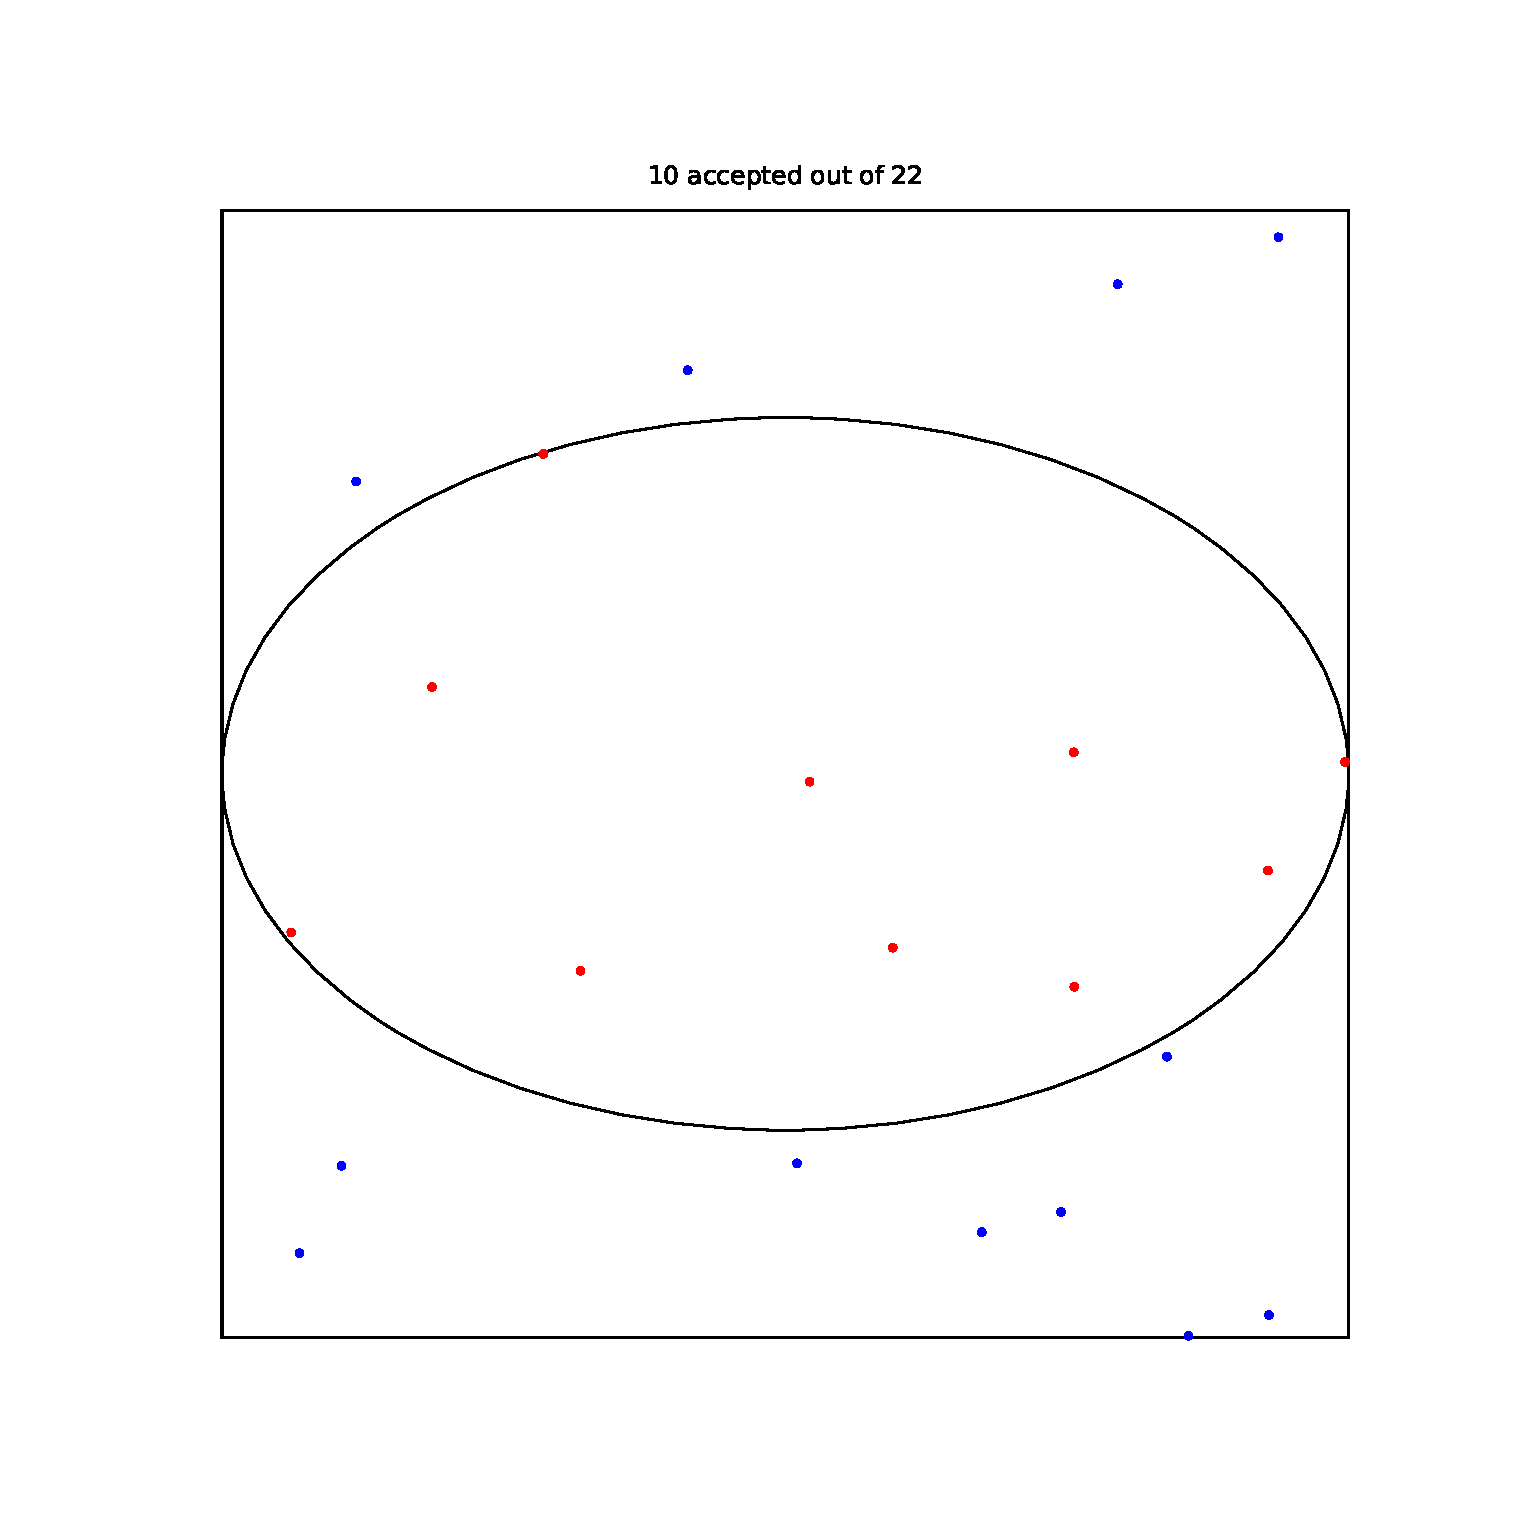
\includegraphics[width=\textwidth, trim=2.7cm 2.7cm 2.7cm 2cm,
        clip]{./points_ellipse_10.eps}
    \end{subfigure}
    \begin{subfigure}{0.45\textwidth}
        \centering
        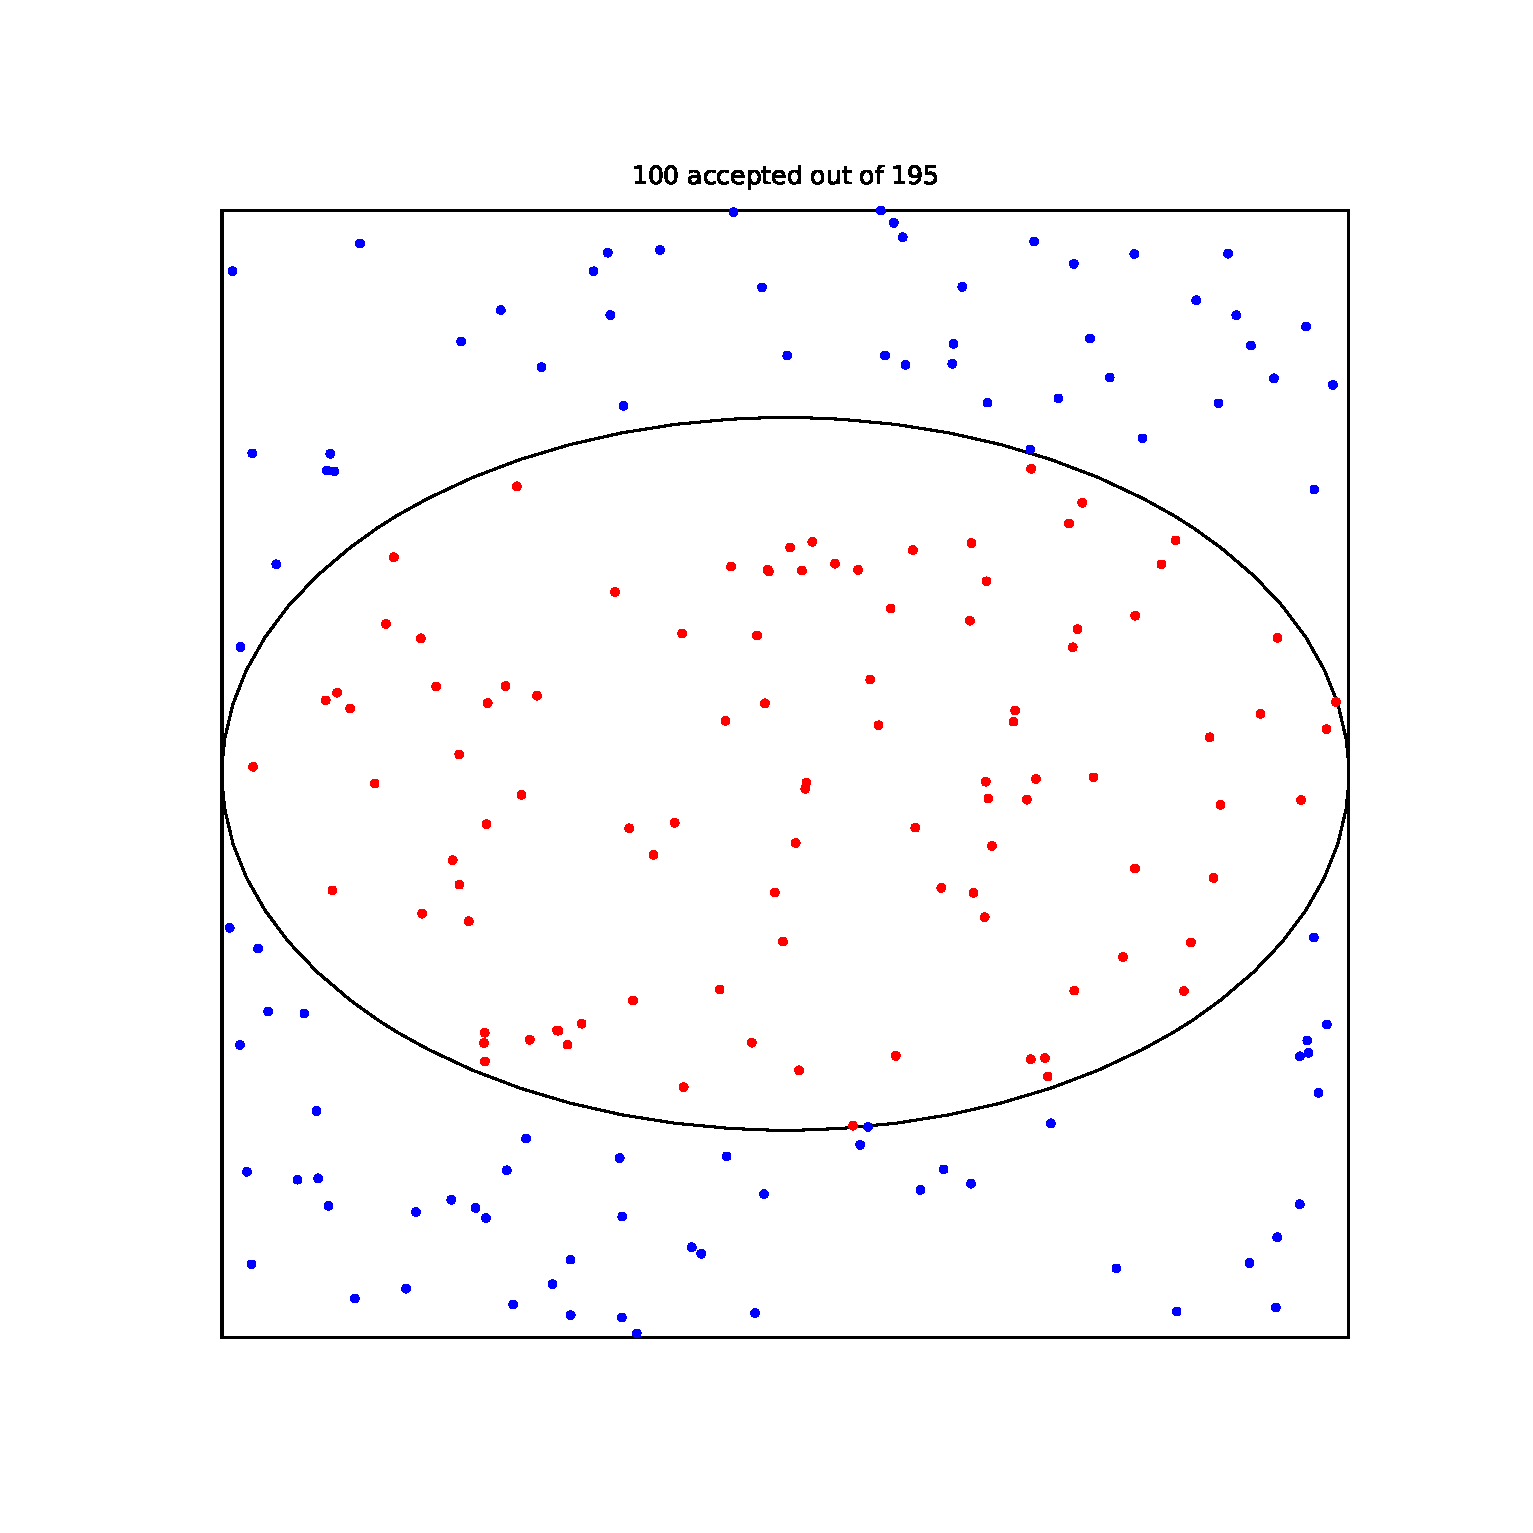
\includegraphics[width=\textwidth, trim=2.7cm 2.7cm 2.7cm 2cm,
        clip]{./points_ellipse_100.eps}
    \end{subfigure}
    \begin{subfigure}{0.45\textwidth}
        \centering
        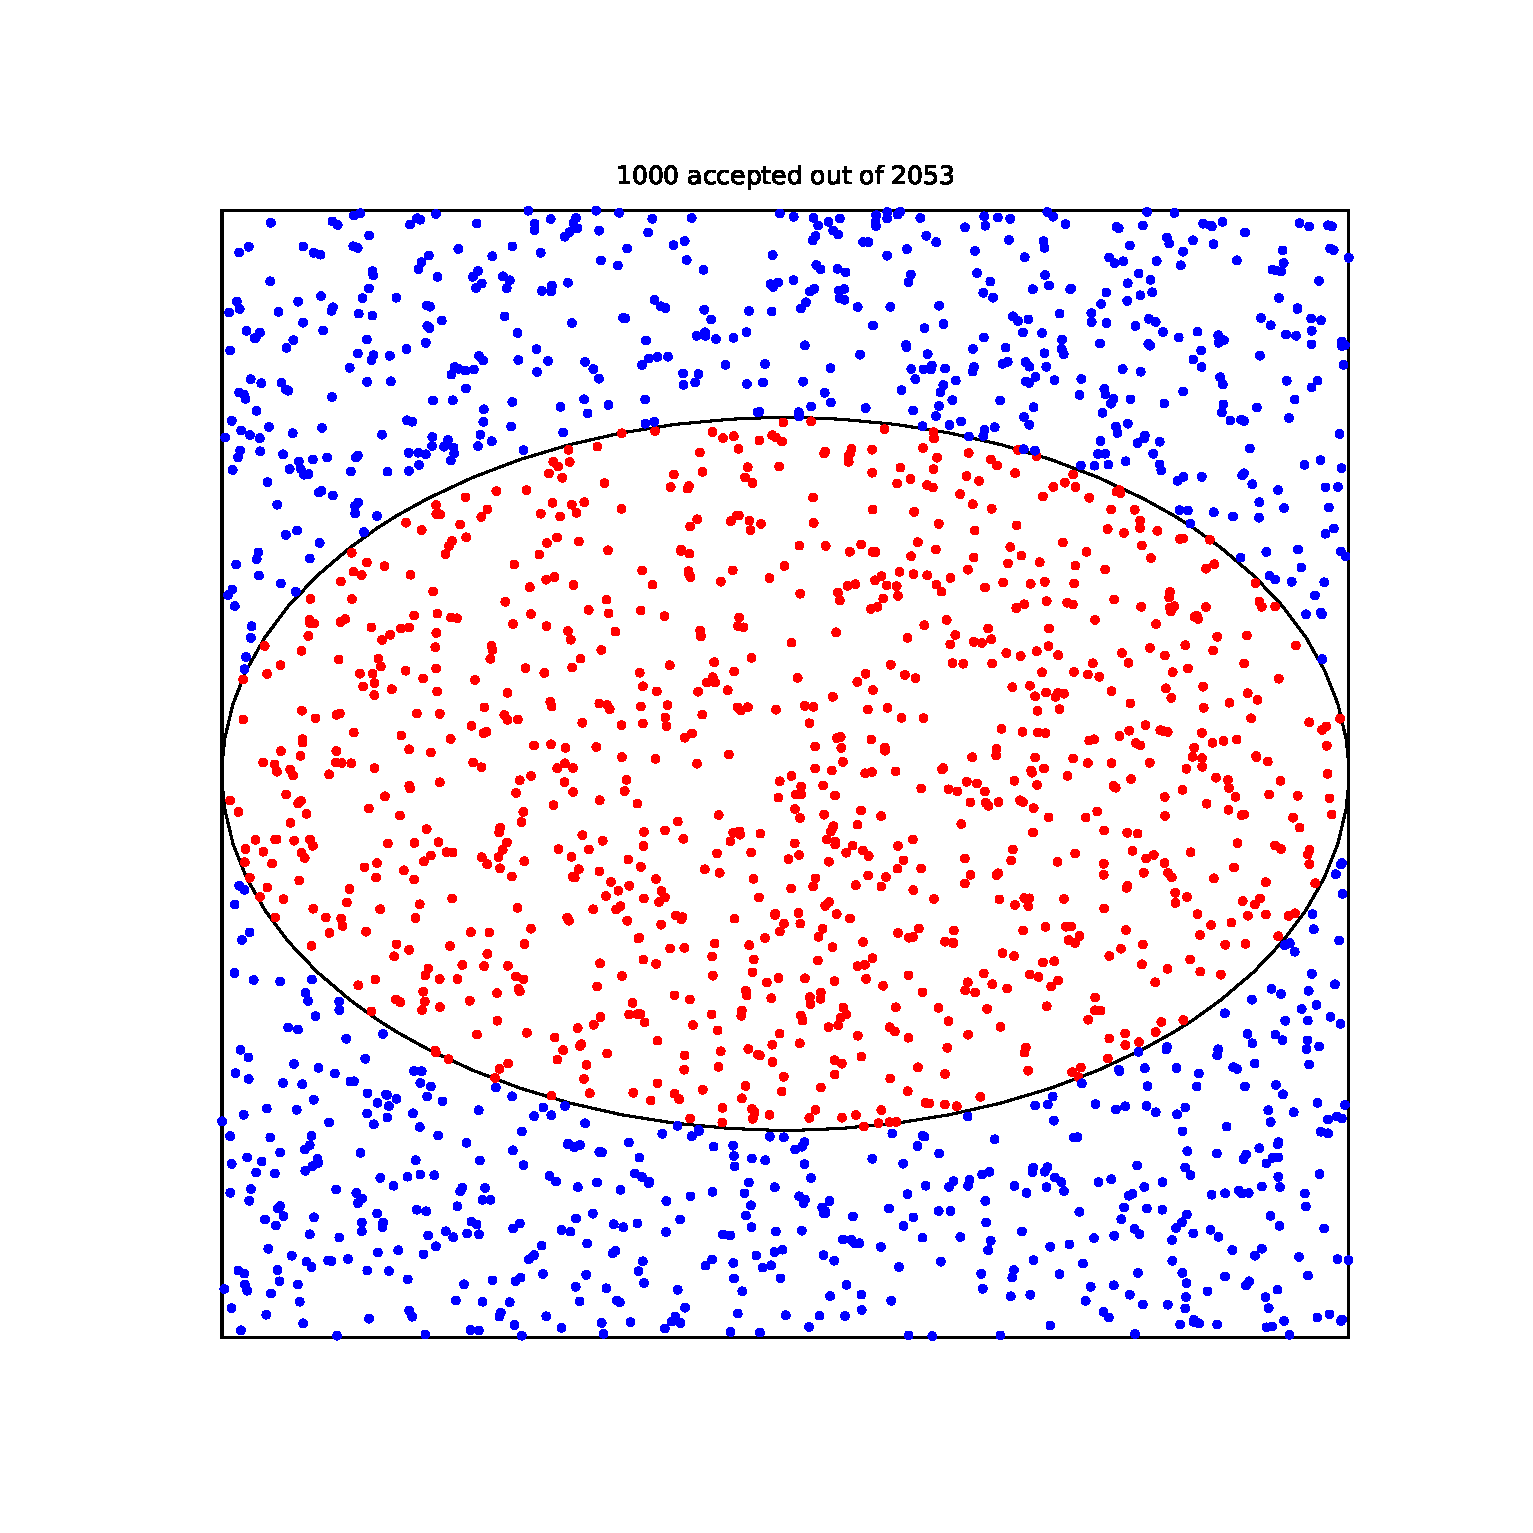
\includegraphics[width=\textwidth, trim=2.7cm 2.7cm 2.7cm 2cm,
        clip]{./points_ellipse_1000.eps}
    \end{subfigure}
    \begin{subfigure}{0.45\textwidth}
        \centering
        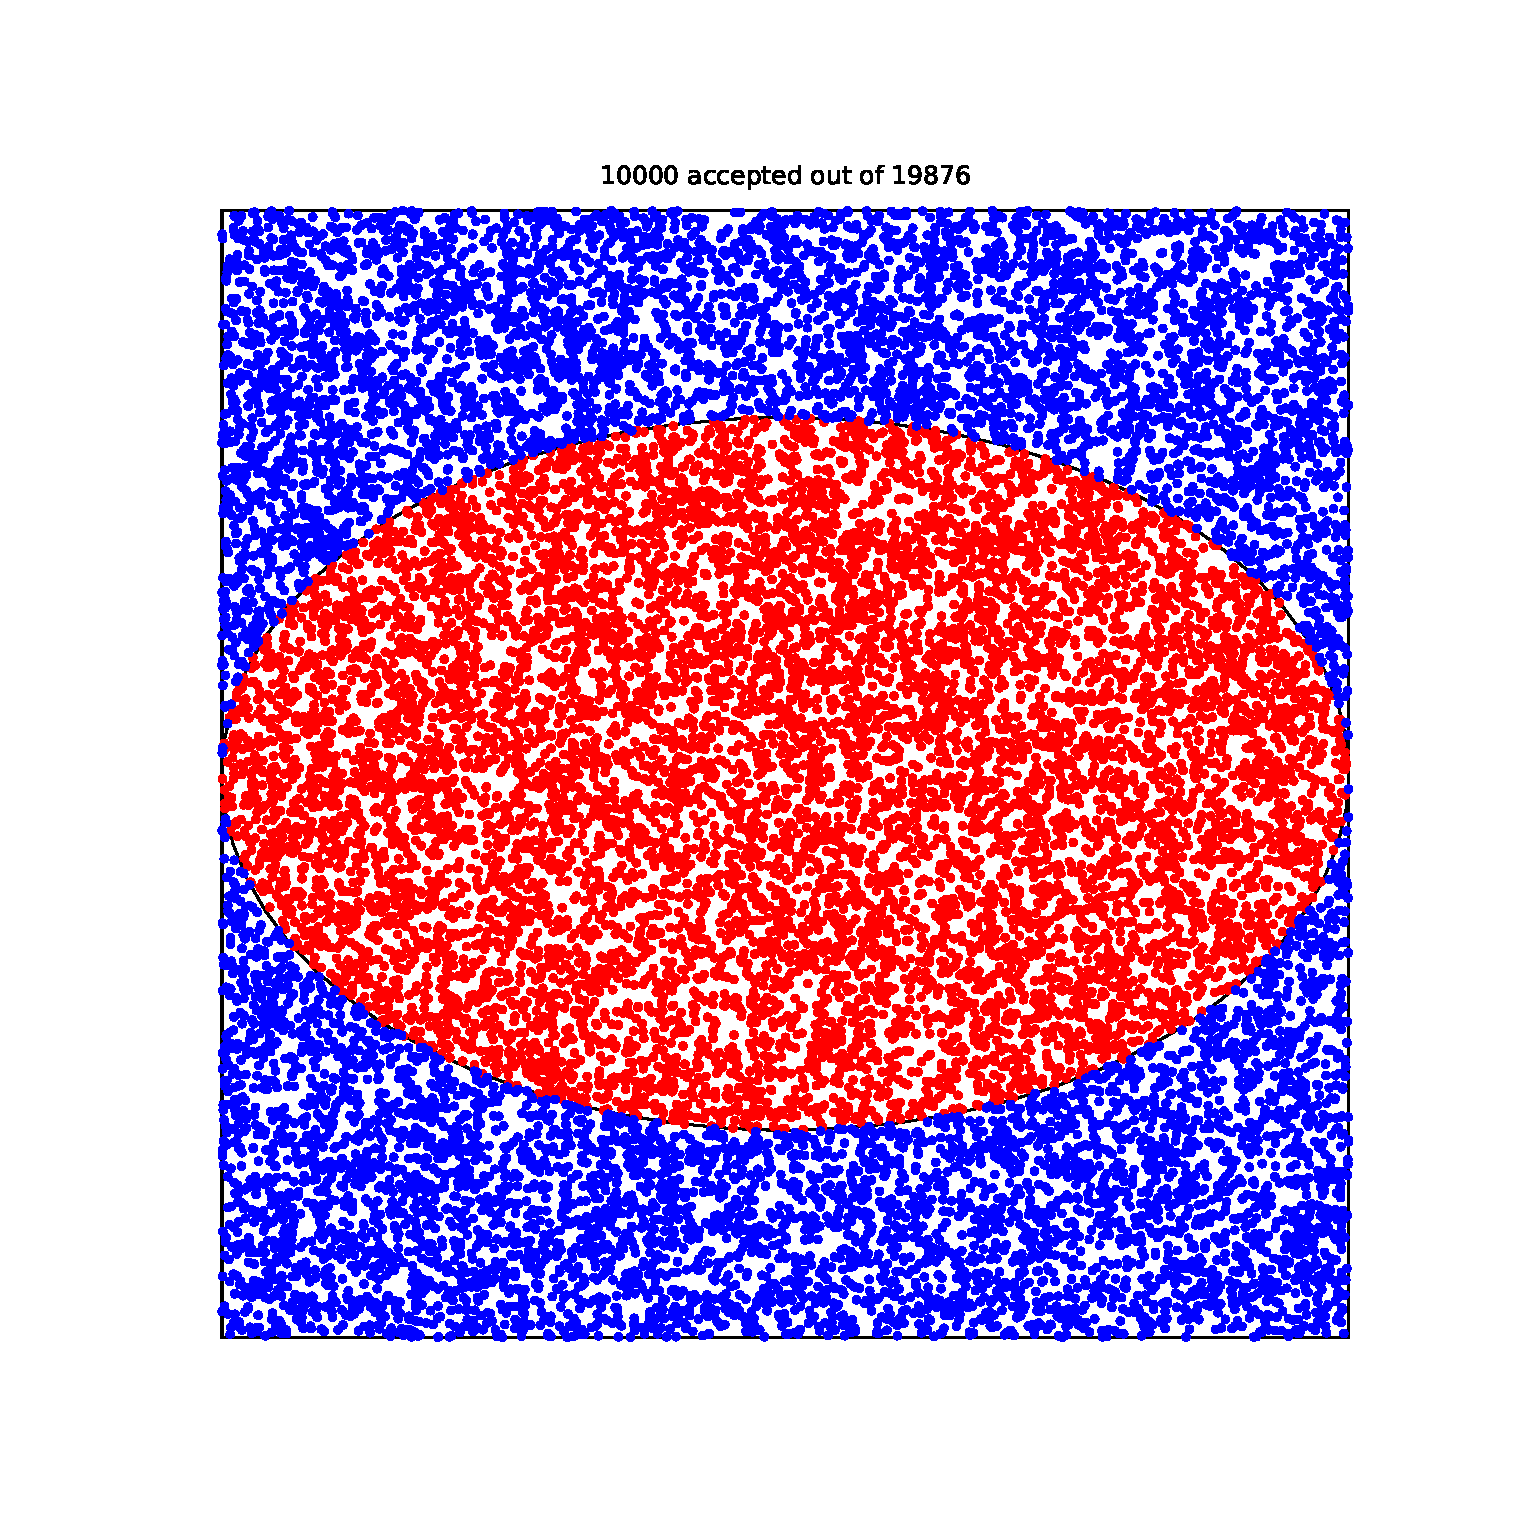
\includegraphics[width=\textwidth, trim=2.7cm 2.7cm 2.7cm 2cm,
        clip]{./points_ellipse_10000.eps}
    \end{subfigure}
    \caption{Samples drawn from the ellipse in red, rejected points in blue, $n =
    10, 100, 1000, 10000$.}
    \end{figure}
    
    Following are executions of the script with $n = 100, 1000, 10^4, 10^5, 10^6$
    samples drawn. The data points have been redirected to separate files for
    brevity.
    
    \begin{lstlisting}[numbers=none, basicstyle=\ttfamily]
        $ ./sample_ellipse.py 100 2> samples_ellipse_100.dat
        100 samples accepted out of 195 draws.
        Estimated value of pi is 3.24336170
        Error is 0.10176905 (3.239409%)
        
        $ ./sample_ellipse.py 1000 2> samples_ellipse_1000.dat
        1000 samples accepted out of 2053 draws.
        Estimated value of pi is 3.08064068
        Error is -0.06095197 (-1.940162%)

        $ ./sample_ellipse.py 10000 2> samples_ellipse_10000.dat
        10000 samples accepted out of 19876 draws.
        Estimated value of pi is 3.18200610
        Error is 0.04041344 (1.286400%)
            
        $ ./sample_ellipse.py 100000 2> samples_ellipse_100000.dat
        100000 samples accepted out of 201676 draws.
        Estimated value of pi is 3.13599800
        Error is -0.00559466 (-0.178083%)

        $ ./sample_ellipse.py 1000000 2> samples_ellipse_1000000.dat
        1000000 samples accepted out of 2012042 draws.
        Estimated value of pi is 3.14335154
        Error is 0.00175889 (0.055987%)
    \end{lstlisting}
    

    \section{Code listings}\label{sec:code_listing}

    \lstinputlisting[language=python, caption=\texttt{sample\_disc.py}]{./sample_disc.py}
    
    \lstinputlisting[language=python,
    caption=\texttt{sample\_disc\_mean.py}]{./sample_disc_mean.py}

    \lstinputlisting[language=python,
    caption=\texttt{sample\_ellipse.py}]{./sample_ellipse.py}
    
    \lstinputlisting[language=c++, caption=\texttt{sample\_disc.cpp}]{./sample_disc.cpp}


\end{document}
